\documentclass{article}
\usepackage{graphicx}
\usepackage{enumitem}
\usepackage{pdfpages}
\usepackage[a4paper, left=1in, right=1in, top=1in, bottom=1in]{geometry}
\usepackage[english]{babel}
\usepackage{fancyhdr}
\pagestyle{fancy}

% Header
\fancyhead[L]{Niklas Fister}
\fancyhead[C]{Kantonnschule Wettingen - Detusch}
\fancyhead[R]{\thepage}


% clear Footer
\fancyfoot{}

% Title
\title{\Huge\textbf{Frauenliteratur}}
\author{Niklas Fister}
\date{\today}

\begin{document}
\maketitle
\thispagestyle{empty}
\newpage

\section{Einführung}
Anhand der Beispieltexten hat man erkannt, dass man den Text von Frauen und Männern nur schwer unterscheiden kann.
Dabei ist der Text "Narzissen für über den Tag" von einer Frau geschrieben, wurde in dem Beispiel jedoch etwas umgeschrieben

\subsection{Frage zur Meinung}
\begin{enumerate}
    \item Was bedeutet Literatur für euch?

    Literatur dient einerseits zur reinen Unterhaltung, jedoch auch zur Bildung. Es macht den Unterschied zwischen die Bücher lediglich geniessen oder sich damit zu befassen.
    \item Wo liegt der Unterschied zur Frauenliteratur?

    Es gibt keinen Unterschied, ausser der Name der Autor:in auf dem Buch. Der Begriff Frauenliteratur ist sehr ungünstig und sollte nicht so existieren. Oftmals wird es mit Literatur assoziiert, welche direkt mit Frauen zu tun hat.
    \item Sollte das Geschlecht eine Rolle spielen, bei dem was wir lesen?

    In fiktionalen Werken macht es keinen Unterschied, jedoch in Büchern, in welchen Geschlechterspezifische Probleme angesprochen werden (gesundheitlich), macht es einen Unterschied.
    \item Wieso behanden wir in der Schule so viele Bücher, die ausschliesslich von männlichen Autoren geschrieben wurden?

    Früher gab es deutlich mehr männliche Autoren, also weibliche. Zudem wurden durch die alte Weltanschauung vor allem Werke männlicher Autoren als essentiell eingestuft. Es liegt somit vor allen an der alten Zeit, der wir noch nachhinken.
    \item Glaubt ihr, es gbit eine gewisse Voreingenommenheit gegenüber Frauen? Wieso?

    Gewisse Menschen sind allgemein gegenüber Frauen voreingenommen und bei diesen wird es so sein. Sachlich fundiert denkende Menschen werden aber nicht solche Gedanken haben. Wir haben immernoch Geschlechterrollen, von denen wir uns aber versuchen zu lösen.
    \item Kann man das Gleichberechtigung nennen?

    Heutzutage sind alle gleich Berechtigt, aber in früheren Zeiten nicht. Somit kommen im Unterricht die Frauen auch oftmals zu kurz, da es von früher zu wenig gibt.
\end{enumerate}

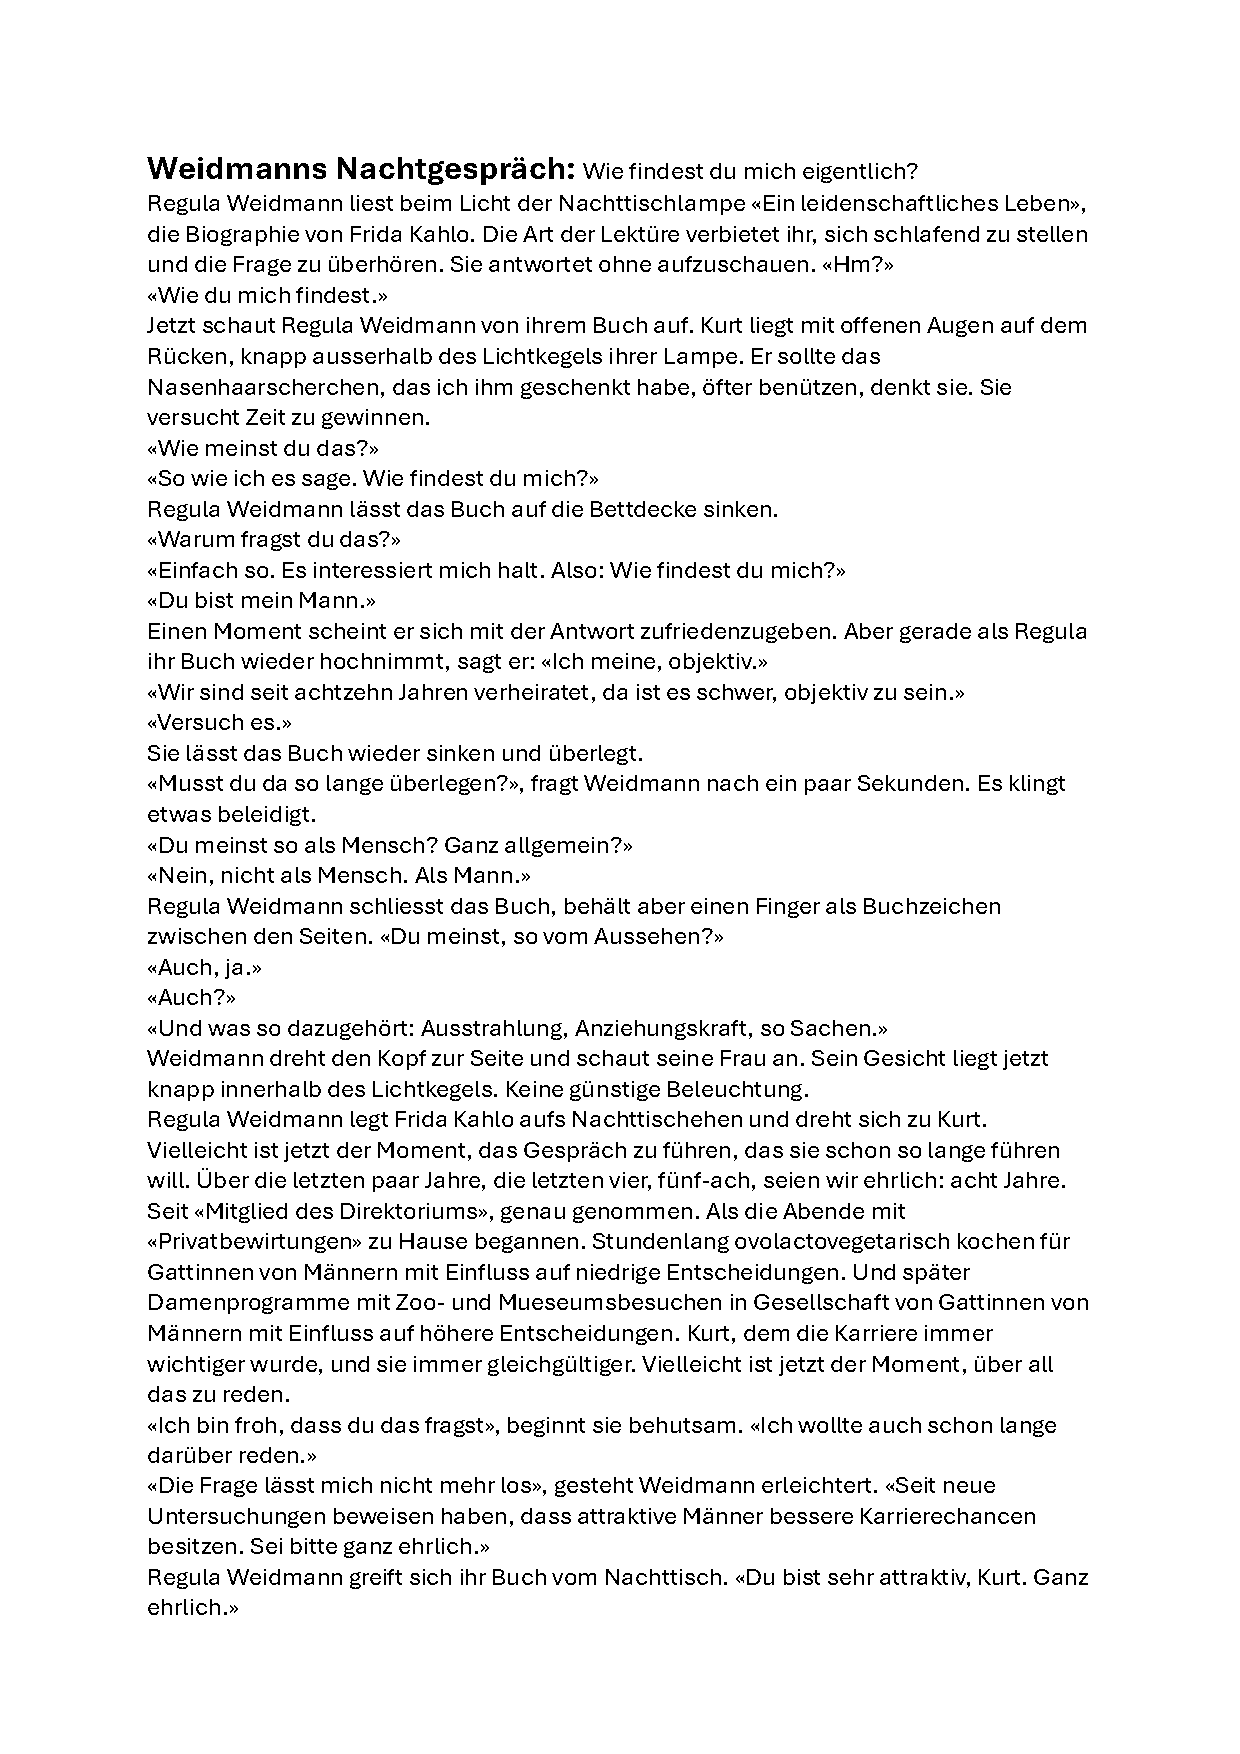
\includepdf[nup=2x1, scale=0.9, pages=-]{resources/pdf/Kurzgeschichten.pdf}

\section{Analyse}
\subsection{Studie Rostock}
Es werden doppelt so häufig Bücher von Frauen geschrieben besprochen werden, wie die von Männern.

Literatur von Männern verfasst spricht oftmals alle an, während Frauenliteratur vor allem Frauen anspricht.

Nominierte Verläge scheinen vorallem auf Männerlitatur zu setzen. Wissenschaftliche Literatur ist mehrheitlich weissen Männern überlassen und Unterhaltung- und Kinderliteratur wird jedoch mehrheiltich von Frauen verfasst. \\

$\rightarrow$ Priviligierte hatten das Recht zu schreiben und das waren zur damaligen Zeit waren das weisse Männerlitatur

Einwand der Verlage war: "Wir achten nicht auf Hautfarbe und Geschlcht, wir gehen nur auf Qualität"

Frauen schrieben vor allem nur Unterhaltungsliteratur, was als schlechter und minderwertiger angesehen wurde.

$\rightarrow$ man hatte schon eine Voreingenommenheit

\subsection{Problem der Frauen}
\begin{itemize}
    \item Rollenklischees
    \item Anzahl Kinder
    \item Äusseres Aussehen

\end{itemize}
$\rightarrow$ Die Rezesion wird oftmals nicht bezüglich des Textes, sondern des Aussehens der Autorin getätigt.\\

Es gibt Zitate wie: "wie ein aufgeschrechtes Reh mit sinlichen Lippen", was die Autorin nur auf ihr äusseres reduziert.

\subsection{Gegenbewegung}

Nadja Bügger, Simone, Meier, Güzerin Kar stellen die Literatur als Geschmackssache dar. Sie kritisieren unter dem Hashtag \textbf{\#dichterdran} Autoren wie Göthe und zeigen, das auch dies als nicht spannend erachtet werden kann.

\paragraph{Aufgabe}
\begin{enumerate}
    \item Was fällt euch and dem Text auf?

    Der Text ist sehr verwerflich und enthält unprofessionelle, abwerdende Kommentare. Lars war ursprünglich mal Laura.
\end{enumerate}

\paragraph{Männliche und weibliche Perspektiven}
\begin{itemize}
    \item Männer schrieben für die Allgemeinheit
    \item Themen der Männer als "Hochwertiger" angesehen
    \item Am Ende lässt sich der Schreibstyle filtern, zwischen Männern und Frauen
    \item Sie sind doch beide ähnlich
    \item Schule gilt als Bildungsquelle und die veraltete Art des Sprachenunterrichts und deren Literatur stärkt die Rollebilder
\end{itemize}

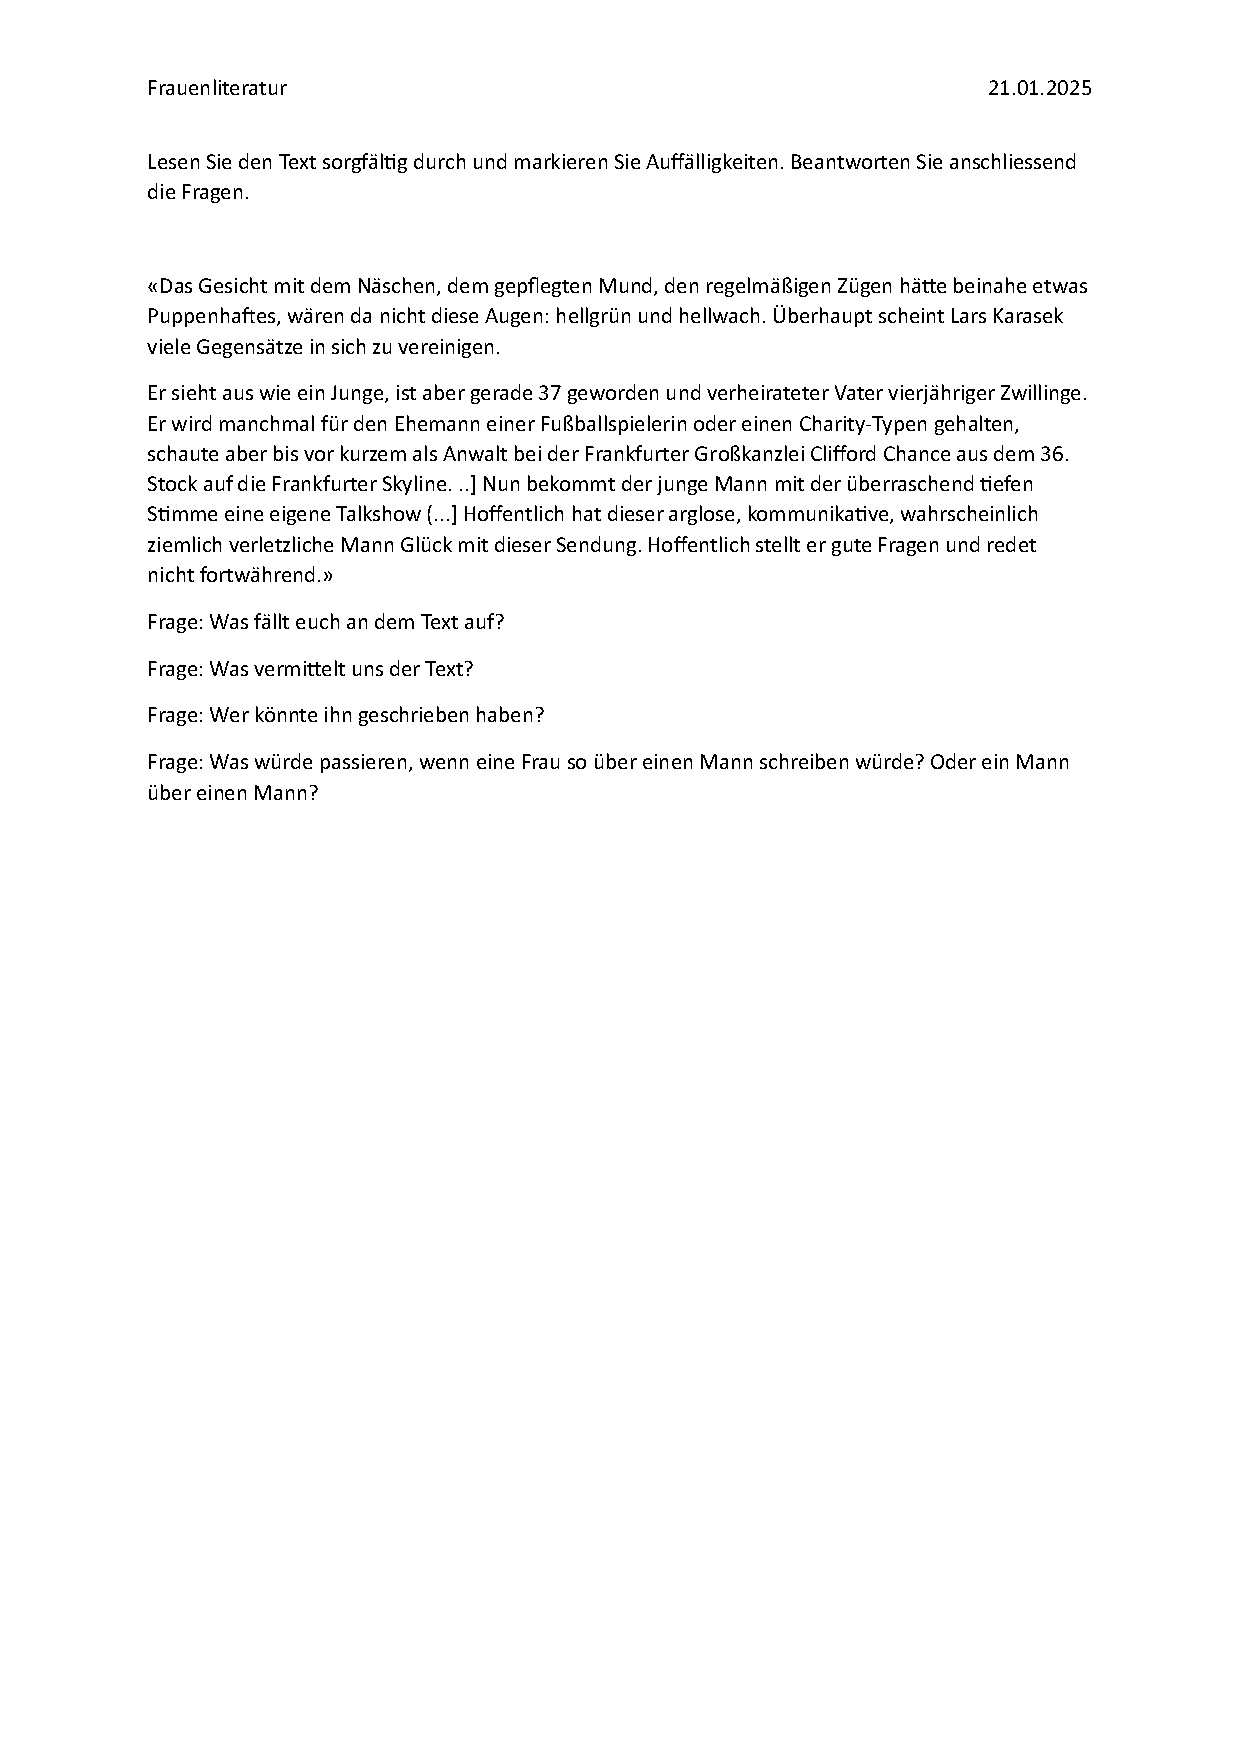
\includepdf[nup=1x1, scale=.9, pages=-]{resources/pdf/Lars_Karasek_Aufgabe.pdf}

\section{Geschichte der Frauenrolle}
\subsection{Mittelalter}
Christine de Pizan (1364-1430) war die erste Frau, die von ihrem Schreiben leben konnte. Sie kritisiert männlichen Autoren, dass sie das Bild der Frau verzerren, um sie ausnützen zu können und damit sie ihnen folgen.

Pizan wird als Feministin von den Männern schwer kritisiert. Jedohc schrieb sie auch Bücher für Männer, wie zum Beispiel ihr Buch für Ritter.
\subsection{Barock}
Sybill Schwarz (1621 - 1568) sie schrieb schon im Alter von 10 Jahren und schrieb in ihrem Leben von 17 Jahren über 200 Gedichte.

Ihre Gedichte wurden als erste Feministische Gedichte eingestuft und sie bekam sogar lob dafür.

\subsection{Aufklärung}
Christiane mariana von Ziegler (1695-1760) schuf mit Bach eine Verbindung zwischen Musik und Literatur.

Sie war die erste Frau des deutschen Vereins für Bildung. Viele waren jedoch gegen ihre Macht. Sie bewiess jedoch wie Frauen die literarische Welt bereichern können.
\end{document}